\documentclass[1p]{elsarticle_modified}
%\bibliographystyle{elsarticle-num}

%\usepackage[colorlinks]{hyperref}
%\usepackage{abbrmath_seonhwa} %\Abb, \Ascr, \Acal ,\Abf, \Afrak
\usepackage{amsfonts}
\usepackage{amssymb}
\usepackage{amsmath}
\usepackage{amsthm}
\usepackage{scalefnt}
\usepackage{amsbsy}
\usepackage{kotex}
\usepackage{caption}
\usepackage{subfig}
\usepackage{color}
\usepackage{graphicx}
\usepackage{xcolor} %% white, black, red, green, blue, cyan, magenta, yellow
\usepackage{float}
\usepackage{setspace}
\usepackage{hyperref}

\usepackage{tikz}
\usetikzlibrary{arrows}

\usepackage{multirow}
\usepackage{array} % fixed length table
\usepackage{hhline}

%%%%%%%%%%%%%%%%%%%%%
\makeatletter
\renewcommand*\env@matrix[1][\arraystretch]{%
	\edef\arraystretch{#1}%
	\hskip -\arraycolsep
	\let\@ifnextchar\new@ifnextchar
	\array{*\c@MaxMatrixCols c}}
\makeatother %https://tex.stackexchange.com/questions/14071/how-can-i-increase-the-line-spacing-in-a-matrix
%%%%%%%%%%%%%%%

\usepackage[normalem]{ulem}

\newcommand{\msout}[1]{\ifmmode\text{\sout{\ensuremath{#1}}}\else\sout{#1}\fi}
%SOURCE: \msout is \stkout macro in https://tex.stackexchange.com/questions/20609/strikeout-in-math-mode

\newcommand{\cancel}[1]{
	\ifmmode
	{\color{red}\msout{#1}}
	\else
	{\color{red}\sout{#1}}
	\fi
}

\newcommand{\add}[1]{
	{\color{blue}\uwave{#1}}
}

\newcommand{\replace}[2]{
	\ifmmode
	{\color{red}\msout{#1}}{\color{blue}\uwave{#2}}
	\else
	{\color{red}\sout{#1}}{\color{blue}\uwave{#2}}
	\fi
}

\newcommand{\Sol}{\mathcal{S}} %segment
\newcommand{\D}{D} %diagram
\newcommand{\A}{\mathcal{A}} %arc


%%%%%%%%%%%%%%%%%%%%%%%%%%%%%5 test

\def\sl{\operatorname{\textup{SL}}(2,\Cbb)}
\def\psl{\operatorname{\textup{PSL}}(2,\Cbb)}
\def\quan{\mkern 1mu \triangleright \mkern 1mu}

\theoremstyle{definition}
\newtheorem{thm}{Theorem}[section]
\newtheorem{prop}[thm]{Proposition}
\newtheorem{lem}[thm]{Lemma}
\newtheorem{ques}[thm]{Question}
\newtheorem{cor}[thm]{Corollary}
\newtheorem{defn}[thm]{Definition}
\newtheorem{exam}[thm]{Example}
\newtheorem{rmk}[thm]{Remark}
\newtheorem{alg}[thm]{Algorithm}

\newcommand{\I}{\sqrt{-1}}
\begin{document}

%\begin{frontmatter}
%
%\title{Boundary parabolic representations of knots up to 8 crossings}
%
%%% Group authors per affiliation:
%\author{Yunhi Cho} 
%\address{Department of Mathematics, University of Seoul, Seoul, Korea}
%\ead{yhcho@uos.ac.kr}
%
%
%\author{Seonhwa Kim} %\fnref{s_kim}}
%\address{Center for Geometry and Physics, Institute for Basic Science, Pohang, 37673, Korea}
%\ead{ryeona17@ibs.re.kr}
%
%\author{Hyuk Kim}
%\address{Department of Mathematical Sciences, Seoul National University, Seoul 08826, Korea}
%\ead{hyukkim@snu.ac.kr}
%
%\author{Seokbeom Yoon}
%\address{Department of Mathematical Sciences, Seoul National University, Seoul, 08826,  Korea}
%\ead{sbyoon15@snu.ac.kr}
%
%\begin{abstract}
%We find all boundary parabolic representation of knots up to 8 crossings.
%
%\end{abstract}
%\begin{keyword}
%    \MSC[2010] 57M25 
%\end{keyword}
%
%\end{frontmatter}

%\linenumbers
%\tableofcontents
%
\newcommand\colored[1]{\textcolor{white}{\rule[-0.35ex]{0.8em}{1.4ex}}\kern-0.8em\color{red} #1}%
%\newcommand\colored[1]{\textcolor{white}{ #1}\kern-2.17ex	\textcolor{white}{ #1}\kern-1.81ex	\textcolor{white}{ #1}\kern-2.15ex\color{red}#1	}

{\Large $\underline{12n_{0496}~(K12n_{0496})}$}

\setlength{\tabcolsep}{10pt}
\renewcommand{\arraystretch}{1.6}
\vspace{1cm}\begin{tabular}{m{100pt}>{\centering\arraybackslash}m{274pt}}
\multirow{5}{120pt}{
	\centering
	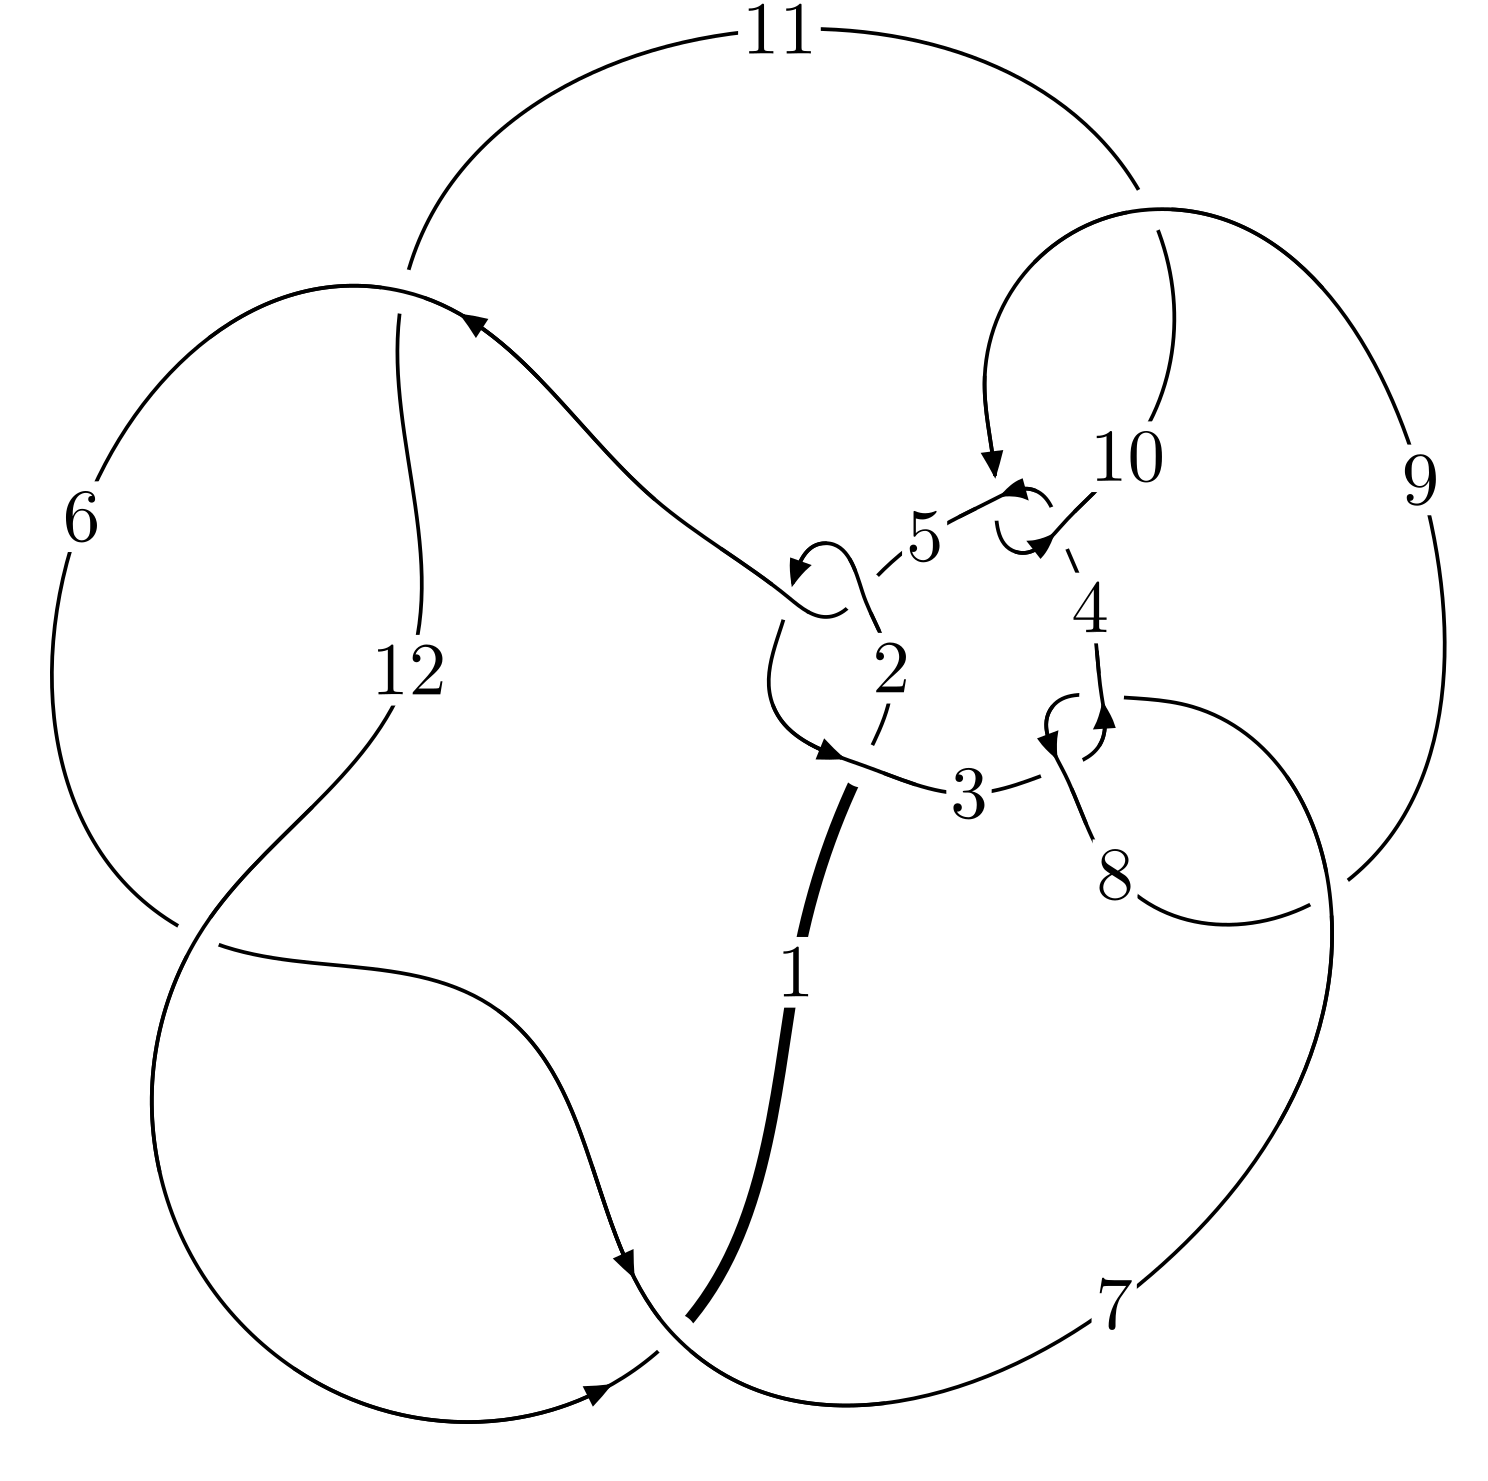
\includegraphics[width=112pt]{../../../GIT/diagram.site/Diagrams/png/2585_12n_0496.png}\\
\ \ \ A knot diagram\footnotemark}&
\allowdisplaybreaks
\textbf{Linearized knot diagam} \\
\cline{2-2}
 &
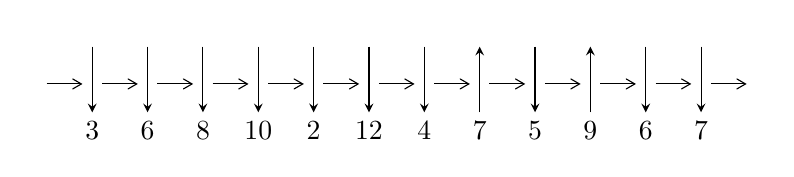
\begin{tikzpicture}[x=20pt, y=17pt]
	% nodes
	\node (C0) at (0, 0) {};
	\node (C1) at (1, 0) {};
	\node (C1U) at (1, +1) {};
	\node (C1D) at (1, -1) {3};

	\node (C2) at (2, 0) {};
	\node (C2U) at (2, +1) {};
	\node (C2D) at (2, -1) {6};

	\node (C3) at (3, 0) {};
	\node (C3U) at (3, +1) {};
	\node (C3D) at (3, -1) {8};

	\node (C4) at (4, 0) {};
	\node (C4U) at (4, +1) {};
	\node (C4D) at (4, -1) {10};

	\node (C5) at (5, 0) {};
	\node (C5U) at (5, +1) {};
	\node (C5D) at (5, -1) {2};

	\node (C6) at (6, 0) {};
	\node (C6U) at (6, +1) {};
	\node (C6D) at (6, -1) {12};

	\node (C7) at (7, 0) {};
	\node (C7U) at (7, +1) {};
	\node (C7D) at (7, -1) {4};

	\node (C8) at (8, 0) {};
	\node (C8U) at (8, +1) {};
	\node (C8D) at (8, -1) {7};

	\node (C9) at (9, 0) {};
	\node (C9U) at (9, +1) {};
	\node (C9D) at (9, -1) {5};

	\node (C10) at (10, 0) {};
	\node (C10U) at (10, +1) {};
	\node (C10D) at (10, -1) {9};

	\node (C11) at (11, 0) {};
	\node (C11U) at (11, +1) {};
	\node (C11D) at (11, -1) {6};

	\node (C12) at (12, 0) {};
	\node (C12U) at (12, +1) {};
	\node (C12D) at (12, -1) {7};
	\node (C13) at (13, 0) {};

	% arrows
	\draw[->,>={angle 60}]
	(C0) edge (C1) (C1) edge (C2) (C2) edge (C3) (C3) edge (C4) (C4) edge (C5) (C5) edge (C6) (C6) edge (C7) (C7) edge (C8) (C8) edge (C9) (C9) edge (C10) (C10) edge (C11) (C11) edge (C12) (C12) edge (C13) ;	\draw[->,>=stealth]
	(C1U) edge (C1D) (C2U) edge (C2D) (C3U) edge (C3D) (C4U) edge (C4D) (C5U) edge (C5D) (C6U) edge (C6D) (C7U) edge (C7D) (C8D) edge (C8U) (C9U) edge (C9D) (C10D) edge (C10U) (C11U) edge (C11D) (C12U) edge (C12D) ;
	\end{tikzpicture} \\
\hhline{~~} \\& 
\textbf{Solving Sequence} \\ \cline{2-2} 
 &
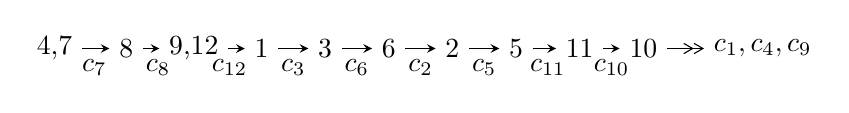
\begin{tikzpicture}[x=23pt, y=7pt]
	% node
	\node (A0) at (-1/8, 0) {4,7};
	\node (A1) at (1, 0) {8};
	\node (A2) at (33/16, 0) {9,12};
	\node (A3) at (25/8, 0) {1};
	\node (A4) at (33/8, 0) {3};
	\node (A5) at (41/8, 0) {6};
	\node (A6) at (49/8, 0) {2};
	\node (A7) at (57/8, 0) {5};
	\node (A8) at (65/8, 0) {11};
	\node (A9) at (73/8, 0) {10};
	\node (C1) at (1/2, -1) {$c_{7}$};
	\node (C2) at (3/2, -1) {$c_{8}$};
	\node (C3) at (21/8, -1) {$c_{12}$};
	\node (C4) at (29/8, -1) {$c_{3}$};
	\node (C5) at (37/8, -1) {$c_{6}$};
	\node (C6) at (45/8, -1) {$c_{2}$};
	\node (C7) at (53/8, -1) {$c_{5}$};
	\node (C8) at (61/8, -1) {$c_{11}$};
	\node (C9) at (69/8, -1) {$c_{10}$};
	\node (A10) at (11, 0) {$c_{1},c_{4},c_{9}$};

	% edge
	\draw[->,>=stealth]	
	(A0) edge (A1) (A1) edge (A2) (A2) edge (A3) (A3) edge (A4) (A4) edge (A5) (A5) edge (A6) (A6) edge (A7) (A7) edge (A8) (A8) edge (A9) ;
	\draw[->>,>={angle 60}]	
	(A9) edge (A10);
\end{tikzpicture} \\ 

\end{tabular} \\

\footnotetext{
The image of knot diagram is generated by the software ``\textbf{Draw programme}" developed by Andrew Bartholomew(\url{http://www.layer8.co.uk/maths/draw/index.htm\#Running-draw}), where we modified some parts for our purpose(\url{https://github.com/CATsTAILs/LinksPainter}).
}\phantom \\ \newline 
\centering \textbf{Ideals for irreducible components\footnotemark of $X_{\text{par}}$} 
 
\begin{align*}
I^u_{1}&=\langle 
3 u^{12}+u^{11}+4 u^{10}-5 u^9+3 u^8- u^7+3 u^6-5 u^5-7 u^4+2 u^2+8 b+8 u+6,\\
\phantom{I^u_{1}}&\phantom{= \langle  }- u^{11}-2 u^9+u^8-4 u^7+u^6-4 u^5+5 u^4-2 u^3+4 u^2+4 a-2 u+2,\\
\phantom{I^u_{1}}&\phantom{= \langle  }u^{13}+3 u^{11}-3 u^{10}+6 u^9-6 u^8+10 u^7-10 u^6+8 u^5-9 u^4+6 u^3-2 u^2+2 u+2\rangle \\
I^u_{2}&=\langle 
-12498270 u^{19}-27347075 u^{18}+\cdots+27481697 b-99369926,\\
\phantom{I^u_{2}}&\phantom{= \langle  }-80173179 u^{19}-177871512 u^{18}+\cdots+274816970 a-993207167,\;u^{20}+3 u^{19}+\cdots+18 u+5\rangle \\
I^u_{3}&=\langle 
- u^6-2 u^4- u^2 a- u^3-2 u^2+b- a- u,\\
\phantom{I^u_{3}}&\phantom{= \langle  }2 u^6 a+2 u^5 a+3 u^6+6 u^4 a+u^5+4 u^3 a+5 u^4+8 u^2 a+4 u^3+2 a^2+4 a u+6 u^2+2 a+u-1,\\
\phantom{I^u_{3}}&\phantom{= \langle  }u^7+2 u^5+u^4+2 u^3+u^2+1\rangle \\
I^u_{4}&=\langle 
b+1,\;- u^2+2 a+u+2,\;u^4+u^2+2\rangle \\
I^u_{5}&=\langle 
- u^{11}+u^{10}-4 u^9+4 u^8-7 u^7+7 u^6-5 u^5+5 u^4- u^2 a- u^3+u^2+b- a,\;2 u^{11}- u^{10}+\cdots+a^2+2,\\
\phantom{I^u_{5}}&\phantom{= \langle  }u^{12}- u^{11}+4 u^{10}-4 u^9+7 u^8-7 u^7+5 u^6-5 u^5+u^4- u^3+1\rangle \\
I^u_{6}&=\langle 
b+u,\;2 a- u+1,\;u^2+1\rangle \\
I^u_{7}&=\langle 
b-1,\;u^3+u^2+2 a+u-3,\;u^4+1\rangle \\
\\
I^v_{1}&=\langle 
a,\;b-1,\;v+1\rangle \\
\end{align*}
\raggedright * 8 irreducible components of $\dim_{\mathbb{C}}=0$, with total 82 representations.\\
\footnotetext{All coefficients of polynomials are rational numbers. But the coefficients are sometimes approximated in decimal forms when there is not enough margin.}
\newpage
\renewcommand{\arraystretch}{1}
\centering \section*{I. $I^u_{1}= \langle 3 u^{12}+u^{11}+\cdots+8 b+6,\;- u^{11}-2 u^9+\cdots+4 a+2,\;u^{13}+3 u^{11}+\cdots+2 u+2 \rangle$}
\flushleft \textbf{(i) Arc colorings}\\
\begin{tabular}{m{7pt} m{180pt} m{7pt} m{180pt} }
\flushright $a_{4}=$&$\begin{pmatrix}0\\u\end{pmatrix}$ \\
\flushright $a_{7}=$&$\begin{pmatrix}1\\0\end{pmatrix}$ \\
\flushright $a_{8}=$&$\begin{pmatrix}1\\u^2\end{pmatrix}$ \\
\flushright $a_{9}=$&$\begin{pmatrix}u^2+1\\u^2\end{pmatrix}$ \\
\flushright $a_{12}=$&$\begin{pmatrix}\frac{1}{4} u^{11}+\frac{1}{2} u^9+\cdots+\frac{1}{2} u-\frac{1}{2}\\-\frac{3}{8} u^{12}-\frac{1}{8} u^{11}+\cdots- u-\frac{3}{4}\end{pmatrix}$ \\
\flushright $a_{1}=$&$\begin{pmatrix}\frac{3}{8} u^{12}+\frac{3}{8} u^{11}+\cdots+\frac{3}{2} u+\frac{1}{4}\\-\frac{3}{8} u^{12}-\frac{1}{8} u^{11}+\cdots- u-\frac{3}{4}\end{pmatrix}$ \\
\flushright $a_{3}=$&$\begin{pmatrix}u\\u^3+u\end{pmatrix}$ \\
\flushright $a_{6}=$&$\begin{pmatrix}\frac{1}{4} u^{11}+\frac{1}{2} u^9+\cdots-\frac{1}{2} u+\frac{1}{2}\\-\frac{3}{8} u^{12}+\frac{3}{8} u^{11}+\cdots-\frac{5}{4} u^2+\frac{1}{4}\end{pmatrix}$ \\
\flushright $a_{2}=$&$\begin{pmatrix}-\frac{1}{4} u^{11}-\frac{1}{2} u^9+\cdots+\frac{1}{2} u-\frac{1}{2}\\-\frac{1}{8} u^{12}-\frac{3}{8} u^{11}+\cdots-\frac{3}{4} u^2-\frac{1}{4}\end{pmatrix}$ \\
\flushright $a_{5}=$&$\begin{pmatrix}- u\\-\frac{1}{2} u^{12}+\frac{1}{2} u^{11}+\cdots+u+1\end{pmatrix}$ \\
\flushright $a_{11}=$&$\begin{pmatrix}- u^4- u^2-1\\-\frac{1}{2} u^{12}-\frac{1}{2} u^{11}+\cdots-2 u-1\end{pmatrix}$ \\
\flushright $a_{10}=$&$\begin{pmatrix}-1\\-\frac{1}{2} u^{12}-\frac{1}{2} u^{11}+\cdots-2 u-1\end{pmatrix}$\\&\end{tabular}
\flushleft \textbf{(ii) Obstruction class $= -1$}\\~\\
\flushleft \textbf{(iii) Cusp Shapes $= \frac{1}{2} u^{12}+\frac{5}{2} u^{11}+\frac{9}{2} u^9-\frac{13}{2} u^8+\frac{21}{2} u^7-\frac{21}{2} u^6+\frac{25}{2} u^5-\frac{39}{2} u^4+10 u^3-9 u^2+8 u-9$}\\~\\
\newpage\renewcommand{\arraystretch}{1}
\flushleft \textbf{(iv) u-Polynomials at the component}\newline \\
\begin{tabular}{m{50pt}|m{274pt}}
Crossings & \hspace{64pt}u-Polynomials at each crossing \\
\hline $$\begin{aligned}c_{1}\end{aligned}$$&$\begin{aligned}
&u^{13}+u^{12}+\cdots+45 u+4
\end{aligned}$\\
\hline $$\begin{aligned}c_{2},c_{5},c_{6}\\c_{11},c_{12}\end{aligned}$$&$\begin{aligned}
&u^{13}+3 u^{12}+\cdots+3 u+2
\end{aligned}$\\
\hline $$\begin{aligned}c_{3},c_{4},c_{7}\\c_{9}\end{aligned}$$&$\begin{aligned}
&u^{13}+3 u^{11}+\cdots+2 u+2
\end{aligned}$\\
\hline $$\begin{aligned}c_{8},c_{10}\end{aligned}$$&$\begin{aligned}
&u^{13}-6 u^{12}+\cdots+12 u+4
\end{aligned}$\\
\hline
\end{tabular}\\~\\
\newpage\renewcommand{\arraystretch}{1}
\flushleft \textbf{(v) Riley Polynomials at the component}\newline \\
\begin{tabular}{m{50pt}|m{274pt}}
Crossings & \hspace{64pt}Riley Polynomials at each crossing \\
\hline $$\begin{aligned}c_{1}\end{aligned}$$&$\begin{aligned}
&y^{13}+11 y^{12}+\cdots+913 y-16
\end{aligned}$\\
\hline $$\begin{aligned}c_{2},c_{5},c_{6}\\c_{11},c_{12}\end{aligned}$$&$\begin{aligned}
&y^{13}- y^{12}+\cdots+45 y-4
\end{aligned}$\\
\hline $$\begin{aligned}c_{3},c_{4},c_{7}\\c_{9}\end{aligned}$$&$\begin{aligned}
&y^{13}+6 y^{12}+\cdots+12 y-4
\end{aligned}$\\
\hline $$\begin{aligned}c_{8},c_{10}\end{aligned}$$&$\begin{aligned}
&y^{13}+6 y^{12}+\cdots+592 y-16
\end{aligned}$\\
\hline
\end{tabular}\\~\\
\newpage\flushleft \textbf{(vi) Complex Volumes and Cusp Shapes}
$$\begin{array}{c|c|c}  
\text{Solutions to }I^u_{1}& \I (\text{vol} + \sqrt{-1}CS) & \text{Cusp shape}\\
 \hline 
\begin{aligned}
u &= \phantom{-}0.929226 + 0.280059 I \\
a &= -1.57901 + 0.35078 I \\
b &= -1.020380 + 0.665255 I\end{aligned}
 & -0.97155 + 5.22971 I & -12.23690 - 3.97423 I \\ \hline\begin{aligned}
u &= \phantom{-}0.929226 - 0.280059 I \\
a &= -1.57901 - 0.35078 I \\
b &= -1.020380 - 0.665255 I\end{aligned}
 & -0.97155 - 5.22971 I & -12.23690 + 3.97423 I \\ \hline\begin{aligned}
u &= \phantom{-}0.167516 + 0.866699 I \\
a &= -0.245529 + 0.584083 I \\
b &= \phantom{-}0.173060 - 1.267070 I\end{aligned}
 & \phantom{-}4.28319 - 0.90080 I & -9.45658 + 7.47152 I \\ \hline\begin{aligned}
u &= \phantom{-}0.167516 - 0.866699 I \\
a &= -0.245529 - 0.584083 I \\
b &= \phantom{-}0.173060 + 1.267070 I\end{aligned}
 & \phantom{-}4.28319 + 0.90080 I & -9.45658 - 7.47152 I \\ \hline\begin{aligned}
u &= \phantom{-}0.796399 + 0.915905 I \\
a &= \phantom{-}1.57817 - 0.32207 I \\
b &= \phantom{-}0.871377 + 0.416192 I\end{aligned}
 & -3.44917 - 7.30520 I & -10.1022 + 10.2949 I \\ \hline\begin{aligned}
u &= \phantom{-}0.796399 - 0.915905 I \\
a &= \phantom{-}1.57817 + 0.32207 I \\
b &= \phantom{-}0.871377 - 0.416192 I\end{aligned}
 & -3.44917 + 7.30520 I & -10.1022 - 10.2949 I \\ \hline\begin{aligned}
u &= -0.369074 + 1.182800 I \\
a &= \phantom{-}0.137445 + 0.036300 I \\
b &= -0.850920 - 1.124830 I\end{aligned}
 & \phantom{-}8.13648 + 2.11284 I & -3.39753 - 3.18179 I \\ \hline\begin{aligned}
u &= -0.369074 - 1.182800 I \\
a &= \phantom{-}0.137445 - 0.036300 I \\
b &= -0.850920 + 1.124830 I\end{aligned}
 & \phantom{-}8.13648 - 2.11284 I & -3.39753 + 3.18179 I \\ \hline\begin{aligned}
u &= -0.741404 + 0.995026 I \\
a &= \phantom{-}1.037390 + 0.553915 I \\
b &= \phantom{-}0.730597 + 0.204654 I\end{aligned}
 & -2.95235 + 4.56373 I & -7.10603 - 0.26574 I \\ \hline\begin{aligned}
u &= -0.741404 - 0.995026 I \\
a &= \phantom{-}1.037390 - 0.553915 I \\
b &= \phantom{-}0.730597 - 0.204654 I\end{aligned}
 & -2.95235 - 4.56373 I & -7.10603 + 0.26574 I\\
 \hline 
 \end{array}$$\newpage$$\begin{array}{c|c|c}  
\text{Solutions to }I^u_{1}& \I (\text{vol} + \sqrt{-1}CS) & \text{Cusp shape}\\
 \hline 
\begin{aligned}
u &= -0.577273 + 1.253670 I \\
a &= -1.44865 - 1.14989 I \\
b &= -1.22052 + 0.78529 I\end{aligned}
 & \phantom{-}5.1437 + 16.4022 I & -7.06197 - 9.59363 I \\ \hline\begin{aligned}
u &= -0.577273 - 1.253670 I \\
a &= -1.44865 + 1.14989 I \\
b &= -1.22052 - 0.78529 I\end{aligned}
 & \phantom{-}5.1437 - 16.4022 I & -7.06197 + 9.59363 I \\ \hline\begin{aligned}
u &= -0.410781\phantom{ +0.000000I} \\
a &= -0.959635\phantom{ +0.000000I} \\
b &= -0.366431\phantom{ +0.000000I}\end{aligned}
 & -0.641398\phantom{ +0.000000I} & -15.2780\phantom{ +0.000000I}\\
 \hline 
 \end{array}$$\newpage\newpage\renewcommand{\arraystretch}{1}
\centering \section*{II. $I^u_{2}= \langle -1.25\times10^{7} u^{19}-2.73\times10^{7} u^{18}+\cdots+2.75\times10^{7} b-9.94\times10^{7},\;-8.02\times10^{7} u^{19}-1.78\times10^{8} u^{18}+\cdots+2.75\times10^{8} a-9.93\times10^{8},\;u^{20}+3 u^{19}+\cdots+18 u+5 \rangle$}
\flushleft \textbf{(i) Arc colorings}\\
\begin{tabular}{m{7pt} m{180pt} m{7pt} m{180pt} }
\flushright $a_{4}=$&$\begin{pmatrix}0\\u\end{pmatrix}$ \\
\flushright $a_{7}=$&$\begin{pmatrix}1\\0\end{pmatrix}$ \\
\flushright $a_{8}=$&$\begin{pmatrix}1\\u^2\end{pmatrix}$ \\
\flushright $a_{9}=$&$\begin{pmatrix}u^2+1\\u^2\end{pmatrix}$ \\
\flushright $a_{12}=$&$\begin{pmatrix}0.291733 u^{19}+0.647236 u^{18}+\cdots+4.92689 u+3.61407\\0.454785 u^{19}+0.995101 u^{18}+\cdots+7.42465 u+3.61586\end{pmatrix}$ \\
\flushright $a_{1}=$&$\begin{pmatrix}-0.163052 u^{19}-0.347865 u^{18}+\cdots-2.49775 u-0.00179062\\0.454785 u^{19}+0.995101 u^{18}+\cdots+7.42465 u+3.61586\end{pmatrix}$ \\
\flushright $a_{3}=$&$\begin{pmatrix}u\\u^3+u\end{pmatrix}$ \\
\flushright $a_{6}=$&$\begin{pmatrix}-0.864463 u^{19}-1.98643 u^{18}+\cdots-16.6818 u-6.40771\\-0.595689 u^{19}-1.29703 u^{18}+\cdots-9.53604 u-3.85004\end{pmatrix}$ \\
\flushright $a_{2}=$&$\begin{pmatrix}-0.653089 u^{19}-1.43379 u^{18}+\cdots-9.37011 u-2.98023\\-0.349978 u^{19}-0.737864 u^{18}+\cdots-3.91291 u-1.28352\end{pmatrix}$ \\
\flushright $a_{5}=$&$\begin{pmatrix}-0.821168 u^{19}-2.00657 u^{18}+\cdots-18.8114 u-8.21548\\-0.621168 u^{19}-1.40657 u^{18}+\cdots-10.8114 u-4.61548\end{pmatrix}$ \\
\flushright $a_{11}=$&$\begin{pmatrix}-0.361356 u^{19}-0.786551 u^{18}+\cdots-5.44322 u+0.633834\\0.104807 u^{19}+0.257238 u^{18}+\cdots+2.51174 u+2.33233\end{pmatrix}$ \\
\flushright $a_{10}=$&$\begin{pmatrix}-0.923097 u^{19}-2.14812 u^{18}+\cdots-14.5205 u-4.80434\\1\end{pmatrix}$\\&\end{tabular}
\flushleft \textbf{(ii) Obstruction class $= -1$}\\~\\
\flushleft \textbf{(iii) Cusp Shapes $= -\frac{7065492}{27481697} u^{19}-\frac{31839998}{27481697} u^{18}+\cdots+\frac{103205694}{27481697} u-\frac{125331692}{27481697}$}\\~\\
\newpage\renewcommand{\arraystretch}{1}
\flushleft \textbf{(iv) u-Polynomials at the component}\newline \\
\begin{tabular}{m{50pt}|m{274pt}}
Crossings & \hspace{64pt}u-Polynomials at each crossing \\
\hline $$\begin{aligned}c_{1}\end{aligned}$$&$\begin{aligned}
&(u^{10}+3 u^9+11 u^8+18 u^7+33 u^6+32 u^5+34 u^4+18 u^3+8 u^2+u+1)^{2}
\end{aligned}$\\
\hline $$\begin{aligned}c_{2},c_{5},c_{6}\\c_{11},c_{12}\end{aligned}$$&$\begin{aligned}
&(u^{10}- u^9- u^8+2 u^7+3 u^6-4 u^5+4 u^3- u+1)^2
\end{aligned}$\\
\hline $$\begin{aligned}c_{3},c_{4},c_{7}\\c_{9}\end{aligned}$$&$\begin{aligned}
&u^{20}+3 u^{19}+\cdots+18 u+5
\end{aligned}$\\
\hline $$\begin{aligned}c_{8},c_{10}\end{aligned}$$&$\begin{aligned}
&u^{20}-11 u^{19}+\cdots-76 u+25
\end{aligned}$\\
\hline
\end{tabular}\\~\\
\newpage\renewcommand{\arraystretch}{1}
\flushleft \textbf{(v) Riley Polynomials at the component}\newline \\
\begin{tabular}{m{50pt}|m{274pt}}
Crossings & \hspace{64pt}Riley Polynomials at each crossing \\
\hline $$\begin{aligned}c_{1}\end{aligned}$$&$\begin{aligned}
&(y^{10}+13 y^9+\cdots+15 y+1)^{2}
\end{aligned}$\\
\hline $$\begin{aligned}c_{2},c_{5},c_{6}\\c_{11},c_{12}\end{aligned}$$&$\begin{aligned}
&(y^{10}-3 y^9+11 y^8-18 y^7+33 y^6-32 y^5+34 y^4-18 y^3+8 y^2- y+1)^{2}
\end{aligned}$\\
\hline $$\begin{aligned}c_{3},c_{4},c_{7}\\c_{9}\end{aligned}$$&$\begin{aligned}
&y^{20}+11 y^{19}+\cdots+76 y+25
\end{aligned}$\\
\hline $$\begin{aligned}c_{8},c_{10}\end{aligned}$$&$\begin{aligned}
&y^{20}-5 y^{19}+\cdots-2276 y+625
\end{aligned}$\\
\hline
\end{tabular}\\~\\
\newpage\flushleft \textbf{(vi) Complex Volumes and Cusp Shapes}
$$\begin{array}{c|c|c}  
\text{Solutions to }I^u_{2}& \I (\text{vol} + \sqrt{-1}CS) & \text{Cusp shape}\\
 \hline 
\begin{aligned}
u &= -0.979461 + 0.188210 I \\
a &= \phantom{-}1.59751 + 0.26897 I \\
b &= \phantom{-}1.142330 + 0.733576 I\end{aligned}
 & \phantom{-}1.87405 - 10.79660 I & -9.84814 + 6.97307 I \\ \hline\begin{aligned}
u &= -0.979461 - 0.188210 I \\
a &= \phantom{-}1.59751 - 0.26897 I \\
b &= \phantom{-}1.142330 - 0.733576 I\end{aligned}
 & \phantom{-}1.87405 + 10.79660 I & -9.84814 - 6.97307 I \\ \hline\begin{aligned}
u &= -0.843090 + 0.709533 I \\
a &= -1.51303 - 0.11033 I \\
b &= -0.773203 + 0.317670 I\end{aligned}
 & -3.82303 + 1.33139 I & -9.94848 - 5.33149 I \\ \hline\begin{aligned}
u &= -0.843090 - 0.709533 I \\
a &= -1.51303 + 0.11033 I \\
b &= -0.773203 - 0.317670 I\end{aligned}
 & -3.82303 - 1.33139 I & -9.94848 + 5.33149 I \\ \hline\begin{aligned}
u &= \phantom{-}0.813642 + 0.789464 I \\
a &= -1.203100 + 0.561936 I \\
b &= -0.773203 + 0.317670 I\end{aligned}
 & -3.82303 + 1.33139 I & -9.94848 - 5.33149 I \\ \hline\begin{aligned}
u &= \phantom{-}0.813642 - 0.789464 I \\
a &= -1.203100 - 0.561936 I \\
b &= -0.773203 - 0.317670 I\end{aligned}
 & -3.82303 - 1.33139 I & -9.94848 + 5.33149 I \\ \hline\begin{aligned}
u &= \phantom{-}0.004473 + 1.188620 I \\
a &= \phantom{-}0.166971 + 0.462136 I \\
b &= \phantom{-}0.351677 - 0.481849 I\end{aligned}
 & \phantom{-}3.14663 + 1.17971 I & -5.77268 - 5.86187 I \\ \hline\begin{aligned}
u &= \phantom{-}0.004473 - 1.188620 I \\
a &= \phantom{-}0.166971 - 0.462136 I \\
b &= \phantom{-}0.351677 + 0.481849 I\end{aligned}
 & \phantom{-}3.14663 - 1.17971 I & -5.77268 + 5.86187 I \\ \hline\begin{aligned}
u &= -0.709802 + 0.215491 I \\
a &= \phantom{-}1.80898 + 0.45664 I \\
b &= \phantom{-}0.794058 + 0.823254 I\end{aligned}
 & \phantom{-}4.23778 - 1.45588 I & -7.02190 + 1.71983 I \\ \hline\begin{aligned}
u &= -0.709802 - 0.215491 I \\
a &= \phantom{-}1.80898 - 0.45664 I \\
b &= \phantom{-}0.794058 - 0.823254 I\end{aligned}
 & \phantom{-}4.23778 + 1.45588 I & -7.02190 - 1.71983 I\\
 \hline 
 \end{array}$$\newpage$$\begin{array}{c|c|c}  
\text{Solutions to }I^u_{2}& \I (\text{vol} + \sqrt{-1}CS) & \text{Cusp shape}\\
 \hline 
\begin{aligned}
u &= -0.540050 + 1.155880 I \\
a &= -1.79606 - 1.06825 I \\
b &= -1.014860 + 0.798709 I\end{aligned}
 & \phantom{-}6.90157 + 6.23908 I & -5.40880 - 5.42921 I \\ \hline\begin{aligned}
u &= -0.540050 - 1.155880 I \\
a &= -1.79606 + 1.06825 I \\
b &= -1.014860 - 0.798709 I\end{aligned}
 & \phantom{-}6.90157 - 6.23908 I & -5.40880 + 5.42921 I \\ \hline\begin{aligned}
u &= \phantom{-}0.256269 + 1.270830 I \\
a &= \phantom{-}0.0612993 + 0.1044580 I \\
b &= \phantom{-}0.794058 - 0.823254 I\end{aligned}
 & \phantom{-}4.23778 + 1.45588 I & -7.02190 - 1.71983 I \\ \hline\begin{aligned}
u &= \phantom{-}0.256269 - 1.270830 I \\
a &= \phantom{-}0.0612993 - 0.1044580 I \\
b &= \phantom{-}0.794058 + 0.823254 I\end{aligned}
 & \phantom{-}4.23778 - 1.45588 I & -7.02190 + 1.71983 I \\ \hline\begin{aligned}
u &= \phantom{-}0.242436 + 0.610608 I \\
a &= \phantom{-}1.73616 + 1.08804 I \\
b &= \phantom{-}0.351677 + 0.481849 I\end{aligned}
 & \phantom{-}3.14663 - 1.17971 I & -5.77268 + 5.86187 I \\ \hline\begin{aligned}
u &= \phantom{-}0.242436 - 0.610608 I \\
a &= \phantom{-}1.73616 - 1.08804 I \\
b &= \phantom{-}0.351677 - 0.481849 I\end{aligned}
 & \phantom{-}3.14663 + 1.17971 I & -5.77268 - 5.86187 I \\ \hline\begin{aligned}
u &= \phantom{-}0.595640 + 1.211330 I \\
a &= \phantom{-}1.53920 - 1.03480 I \\
b &= \phantom{-}1.142330 + 0.733576 I\end{aligned}
 & \phantom{-}1.87405 - 10.79660 I & -9.84814 + 6.97307 I \\ \hline\begin{aligned}
u &= \phantom{-}0.595640 - 1.211330 I \\
a &= \phantom{-}1.53920 + 1.03480 I \\
b &= \phantom{-}1.142330 - 0.733576 I\end{aligned}
 & \phantom{-}1.87405 + 10.79660 I & -9.84814 - 6.97307 I \\ \hline\begin{aligned}
u &= -0.340059 + 1.345340 I \\
a &= -0.0979292 - 0.0498685 I \\
b &= -1.014860 - 0.798709 I\end{aligned}
 & \phantom{-}6.90157 - 6.23908 I & -5.40880 + 5.42921 I \\ \hline\begin{aligned}
u &= -0.340059 - 1.345340 I \\
a &= -0.0979292 + 0.0498685 I \\
b &= -1.014860 + 0.798709 I\end{aligned}
 & \phantom{-}6.90157 + 6.23908 I & -5.40880 - 5.42921 I\\
 \hline 
 \end{array}$$\newpage\newpage\renewcommand{\arraystretch}{1}
\centering \section*{III. $I^u_{3}= \langle - u^6-2 u^4- u^2 a- u^3-2 u^2+b- a- u,\;2 u^6 a+3 u^6+\cdots+2 a-1,\;u^7+2 u^5+u^4+2 u^3+u^2+1 \rangle$}
\flushleft \textbf{(i) Arc colorings}\\
\begin{tabular}{m{7pt} m{180pt} m{7pt} m{180pt} }
\flushright $a_{4}=$&$\begin{pmatrix}0\\u\end{pmatrix}$ \\
\flushright $a_{7}=$&$\begin{pmatrix}1\\0\end{pmatrix}$ \\
\flushright $a_{8}=$&$\begin{pmatrix}1\\u^2\end{pmatrix}$ \\
\flushright $a_{9}=$&$\begin{pmatrix}u^2+1\\u^2\end{pmatrix}$ \\
\flushright $a_{12}=$&$\begin{pmatrix}a\\u^6+2 u^4+u^2 a+u^3+2 u^2+a+u\end{pmatrix}$ \\
\flushright $a_{1}=$&$\begin{pmatrix}- u^6-2 u^4- u^2 a- u^3-2 u^2- u\\u^6+2 u^4+u^2 a+u^3+2 u^2+a+u\end{pmatrix}$ \\
\flushright $a_{3}=$&$\begin{pmatrix}u\\u^3+u\end{pmatrix}$ \\
\flushright $a_{6}=$&$\begin{pmatrix}u^6 a+u^6+2 u^4 a+2 u^4+2 u^2 a+2 u^2- u\\- u^5 a+u^6-2 u^3 a+2 u^4- a u+2 u^2\end{pmatrix}$ \\
\flushright $a_{2}=$&$\begin{pmatrix}- u^6 a- u^6-2 u^4 a-2 u^4-2 u^2 a-2 u^2+u\\- u^6 a+u^5 a+u^6- u^4 a+u^5+u^3 a+2 u^4+4 u^3+a u+2 u^2+a+3 u\end{pmatrix}$ \\
\flushright $a_{5}=$&$\begin{pmatrix}- u\\- u^6+u^5- u^4+1\end{pmatrix}$ \\
\flushright $a_{11}=$&$\begin{pmatrix}- u^4- u^2-1\\- u^6- u^5-2 u^4-2 u^3-2 u^2- u-1\end{pmatrix}$ \\
\flushright $a_{10}=$&$\begin{pmatrix}-1\\- u^6- u^5- u^4-2 u^3-2 u^2- u-1\end{pmatrix}$\\&\end{tabular}
\flushleft \textbf{(ii) Obstruction class $= -1$}\\~\\
\flushleft \textbf{(iii) Cusp Shapes $= 4 u^6+4 u^5+4 u^4+8 u^3+8 u^2+4 u-10$}\\~\\
\newpage\renewcommand{\arraystretch}{1}
\flushleft \textbf{(iv) u-Polynomials at the component}\newline \\
\begin{tabular}{m{50pt}|m{274pt}}
Crossings & \hspace{64pt}u-Polynomials at each crossing \\
\hline $$\begin{aligned}c_{1}\end{aligned}$$&$\begin{aligned}
&u^{14}+7 u^{13}+\cdots+254 u+121
\end{aligned}$\\
\hline $$\begin{aligned}c_{2},c_{5},c_{6}\\c_{11},c_{12}\end{aligned}$$&$\begin{aligned}
&u^{14}+3 u^{13}+\cdots+34 u+11
\end{aligned}$\\
\hline $$\begin{aligned}c_{3},c_{4},c_{7}\\c_{9}\end{aligned}$$&$\begin{aligned}
&(u^7+2 u^5+u^4+2 u^3+u^2+1)^2
\end{aligned}$\\
\hline $$\begin{aligned}c_{8},c_{10}\end{aligned}$$&$\begin{aligned}
&(u^7-4 u^6+8 u^5-7 u^4+2 u^3+3 u^2-2 u+1)^2
\end{aligned}$\\
\hline
\end{tabular}\\~\\
\newpage\renewcommand{\arraystretch}{1}
\flushleft \textbf{(v) Riley Polynomials at the component}\newline \\
\begin{tabular}{m{50pt}|m{274pt}}
Crossings & \hspace{64pt}Riley Polynomials at each crossing \\
\hline $$\begin{aligned}c_{1}\end{aligned}$$&$\begin{aligned}
&y^{14}+y^{13}+\cdots+56242 y+14641
\end{aligned}$\\
\hline $$\begin{aligned}c_{2},c_{5},c_{6}\\c_{11},c_{12}\end{aligned}$$&$\begin{aligned}
&y^{14}-7 y^{13}+\cdots-254 y+121
\end{aligned}$\\
\hline $$\begin{aligned}c_{3},c_{4},c_{7}\\c_{9}\end{aligned}$$&$\begin{aligned}
&(y^7+4 y^6+8 y^5+7 y^4+2 y^3-3 y^2-2 y-1)^2
\end{aligned}$\\
\hline $$\begin{aligned}c_{8},c_{10}\end{aligned}$$&$\begin{aligned}
&(y^7+12 y^5+3 y^4+22 y^3-3 y^2-2 y-1)^2
\end{aligned}$\\
\hline
\end{tabular}\\~\\
\newpage\flushleft \textbf{(vi) Complex Volumes and Cusp Shapes}
$$\begin{array}{c|c|c}  
\text{Solutions to }I^u_{3}& \I (\text{vol} + \sqrt{-1}CS) & \text{Cusp shape}\\
 \hline 
\begin{aligned}
u &= -0.468927 + 1.008510 I \\
a &= -0.137111 - 0.945771 I \\
b &= -0.543255 + 0.753172 I\end{aligned}
 & -1.13946 + 6.00484 I & -7.73392 - 8.08638 I \\ \hline\begin{aligned}
u &= -0.468927 + 1.008510 I \\
a &= \phantom{-}1.15206 + 0.83449 I \\
b &= \phantom{-}1.402030 - 0.105113 I\end{aligned}
 & -1.13946 + 6.00484 I & -7.73392 - 8.08638 I \\ \hline\begin{aligned}
u &= -0.468927 - 1.008510 I \\
a &= -0.137111 + 0.945771 I \\
b &= -0.543255 - 0.753172 I\end{aligned}
 & -1.13946 - 6.00484 I & -7.73392 + 8.08638 I \\ \hline\begin{aligned}
u &= -0.468927 - 1.008510 I \\
a &= \phantom{-}1.15206 - 0.83449 I \\
b &= \phantom{-}1.402030 + 0.105113 I\end{aligned}
 & -1.13946 - 6.00484 I & -7.73392 + 8.08638 I \\ \hline\begin{aligned}
u &= -0.824481\phantom{ +0.000000I} \\
a &= -1.134300 + 0.394235 I \\
b &= -0.692469 + 0.662223 I\end{aligned}
 & \phantom{-}0.0577569\phantom{ +0.000000I} & -10.7630\phantom{ +0.000000I} \\ \hline\begin{aligned}
u &= -0.824481\phantom{ +0.000000I} \\
a &= -1.134300 - 0.394235 I \\
b &= -0.692469 - 0.662223 I\end{aligned}
 & \phantom{-}0.0577569\phantom{ +0.000000I} & -10.7630\phantom{ +0.000000I} \\ \hline\begin{aligned}
u &= \phantom{-}0.391915 + 0.631080 I \\
a &= -0.915562 - 0.479802 I \\
b &= -1.164390 + 0.328250 I\end{aligned}
 & -3.69786 - 1.46776 I & -13.4123 + 4.8542 I \\ \hline\begin{aligned}
u &= \phantom{-}0.391915 + 0.631080 I \\
a &= \phantom{-}1.23572 - 1.87006 I \\
b &= \phantom{-}1.148250 + 0.342291 I\end{aligned}
 & -3.69786 - 1.46776 I & -13.4123 + 4.8542 I \\ \hline\begin{aligned}
u &= \phantom{-}0.391915 - 0.631080 I \\
a &= -0.915562 + 0.479802 I \\
b &= -1.164390 - 0.328250 I\end{aligned}
 & -3.69786 + 1.46776 I & -13.4123 - 4.8542 I \\ \hline\begin{aligned}
u &= \phantom{-}0.391915 - 0.631080 I \\
a &= \phantom{-}1.23572 + 1.87006 I \\
b &= \phantom{-}1.148250 - 0.342291 I\end{aligned}
 & -3.69786 + 1.46776 I & -13.4123 - 4.8542 I\\
 \hline 
 \end{array}$$\newpage$$\begin{array}{c|c|c}  
\text{Solutions to }I^u_{3}& \I (\text{vol} + \sqrt{-1}CS) & \text{Cusp shape}\\
 \hline 
\begin{aligned}
u &= \phantom{-}0.489252 + 1.239920 I \\
a &= -1.10571 + 0.94503 I \\
b &= -1.09240 - 0.92531 I\end{aligned}
 & \phantom{-}7.27584 - 9.47458 I & -4.47246 + 6.21855 I \\ \hline\begin{aligned}
u &= \phantom{-}0.489252 + 1.239920 I \\
a &= \phantom{-}0.404899 + 0.133299 I \\
b &= -0.557760 + 1.149380 I\end{aligned}
 & \phantom{-}7.27584 - 9.47458 I & -4.47246 + 6.21855 I \\ \hline\begin{aligned}
u &= \phantom{-}0.489252 - 1.239920 I \\
a &= -1.10571 - 0.94503 I \\
b &= -1.09240 + 0.92531 I\end{aligned}
 & \phantom{-}7.27584 + 9.47458 I & -4.47246 - 6.21855 I \\ \hline\begin{aligned}
u &= \phantom{-}0.489252 - 1.239920 I \\
a &= \phantom{-}0.404899 - 0.133299 I \\
b &= -0.557760 - 1.149380 I\end{aligned}
 & \phantom{-}7.27584 + 9.47458 I & -4.47246 - 6.21855 I\\
 \hline 
 \end{array}$$\newpage\newpage\renewcommand{\arraystretch}{1}
\centering \section*{IV. $I^u_{4}= \langle b+1,\;- u^2+2 a+u+2,\;u^4+u^2+2 \rangle$}
\flushleft \textbf{(i) Arc colorings}\\
\begin{tabular}{m{7pt} m{180pt} m{7pt} m{180pt} }
\flushright $a_{4}=$&$\begin{pmatrix}0\\u\end{pmatrix}$ \\
\flushright $a_{7}=$&$\begin{pmatrix}1\\0\end{pmatrix}$ \\
\flushright $a_{8}=$&$\begin{pmatrix}1\\u^2\end{pmatrix}$ \\
\flushright $a_{9}=$&$\begin{pmatrix}u^2+1\\u^2\end{pmatrix}$ \\
\flushright $a_{12}=$&$\begin{pmatrix}\frac{1}{2} u^2-\frac{1}{2} u-1\\-1\end{pmatrix}$ \\
\flushright $a_{1}=$&$\begin{pmatrix}\frac{1}{2} u^2-\frac{1}{2} u\\-1\end{pmatrix}$ \\
\flushright $a_{3}=$&$\begin{pmatrix}u\\u^3+u\end{pmatrix}$ \\
\flushright $a_{6}=$&$\begin{pmatrix}\frac{1}{2} u^2-\frac{1}{2} u\\-1\end{pmatrix}$ \\
\flushright $a_{2}=$&$\begin{pmatrix}\frac{1}{2} u^2+\frac{1}{2} u\\u^3+u-1\end{pmatrix}$ \\
\flushright $a_{5}=$&$\begin{pmatrix}- u\\- u^3- u\end{pmatrix}$ \\
\flushright $a_{11}=$&$\begin{pmatrix}-1\\0\end{pmatrix}$ \\
\flushright $a_{10}=$&$\begin{pmatrix}1\\u^2+2\end{pmatrix}$\\&\end{tabular}
\flushleft \textbf{(ii) Obstruction class $= 1$}\\~\\
\flushleft \textbf{(iii) Cusp Shapes $= 4 u^2-12$}\\~\\
\newpage\renewcommand{\arraystretch}{1}
\flushleft \textbf{(iv) u-Polynomials at the component}\newline \\
\begin{tabular}{m{50pt}|m{274pt}}
Crossings & \hspace{64pt}u-Polynomials at each crossing \\
\hline $$\begin{aligned}c_{1},c_{5},c_{11}\\c_{12}\end{aligned}$$&$\begin{aligned}
&(u-1)^4
\end{aligned}$\\
\hline $$\begin{aligned}c_{2},c_{6}\end{aligned}$$&$\begin{aligned}
&(u+1)^4
\end{aligned}$\\
\hline $$\begin{aligned}c_{3},c_{4},c_{7}\\c_{9}\end{aligned}$$&$\begin{aligned}
&u^4+u^2+2
\end{aligned}$\\
\hline $$\begin{aligned}c_{8},c_{10}\end{aligned}$$&$\begin{aligned}
&(u^2- u+2)^2
\end{aligned}$\\
\hline
\end{tabular}\\~\\
\newpage\renewcommand{\arraystretch}{1}
\flushleft \textbf{(v) Riley Polynomials at the component}\newline \\
\begin{tabular}{m{50pt}|m{274pt}}
Crossings & \hspace{64pt}Riley Polynomials at each crossing \\
\hline $$\begin{aligned}c_{1},c_{2},c_{5}\\c_{6},c_{11},c_{12}\end{aligned}$$&$\begin{aligned}
&(y-1)^4
\end{aligned}$\\
\hline $$\begin{aligned}c_{3},c_{4},c_{7}\\c_{9}\end{aligned}$$&$\begin{aligned}
&(y^2+y+2)^2
\end{aligned}$\\
\hline $$\begin{aligned}c_{8},c_{10}\end{aligned}$$&$\begin{aligned}
&(y^2+3 y+4)^2
\end{aligned}$\\
\hline
\end{tabular}\\~\\
\newpage\flushleft \textbf{(vi) Complex Volumes and Cusp Shapes}
$$\begin{array}{c|c|c}  
\text{Solutions to }I^u_{4}& \I (\text{vol} + \sqrt{-1}CS) & \text{Cusp shape}\\
 \hline 
\begin{aligned}
u &= \phantom{-}0.676097 + 0.978318 I \\
a &= -1.58805 + 0.17228 I \\
b &= -1.00000\phantom{ +0.000000I}\end{aligned}
 & -4.11234 - 5.33349 I & -14.0000 + 5.2915 I \\ \hline\begin{aligned}
u &= \phantom{-}0.676097 - 0.978318 I \\
a &= -1.58805 - 0.17228 I \\
b &= -1.00000\phantom{ +0.000000I}\end{aligned}
 & -4.11234 + 5.33349 I & -14.0000 - 5.2915 I \\ \hline\begin{aligned}
u &= -0.676097 + 0.978318 I \\
a &= -0.91195 - 1.15060 I \\
b &= -1.00000\phantom{ +0.000000I}\end{aligned}
 & -4.11234 + 5.33349 I & -14.0000 - 5.2915 I \\ \hline\begin{aligned}
u &= -0.676097 - 0.978318 I \\
a &= -0.91195 + 1.15060 I \\
b &= -1.00000\phantom{ +0.000000I}\end{aligned}
 & -4.11234 - 5.33349 I & -14.0000 + 5.2915 I\\
 \hline 
 \end{array}$$\newpage\newpage\renewcommand{\arraystretch}{1}
\centering \section*{V. $I^u_{5}= \langle - u^{11}+u^{10}+\cdots+b- a,\;2 u^{11}- u^{10}+\cdots+a^2+2,\;u^{12}- u^{11}+\cdots- u^3+1 \rangle$}
\flushleft \textbf{(i) Arc colorings}\\
\begin{tabular}{m{7pt} m{180pt} m{7pt} m{180pt} }
\flushright $a_{4}=$&$\begin{pmatrix}0\\u\end{pmatrix}$ \\
\flushright $a_{7}=$&$\begin{pmatrix}1\\0\end{pmatrix}$ \\
\flushright $a_{8}=$&$\begin{pmatrix}1\\u^2\end{pmatrix}$ \\
\flushright $a_{9}=$&$\begin{pmatrix}u^2+1\\u^2\end{pmatrix}$ \\
\flushright $a_{12}=$&$\begin{pmatrix}a\\u^{11}- u^{10}+4 u^9-4 u^8+7 u^7-7 u^6+5 u^5-5 u^4+u^2 a+u^3- u^2+a\end{pmatrix}$ \\
\flushright $a_{1}=$&$\begin{pmatrix}- u^{11}+u^{10}-4 u^9+4 u^8-7 u^7+7 u^6-5 u^5+5 u^4- u^2 a- u^3+u^2\\u^{11}- u^{10}+4 u^9-4 u^8+7 u^7-7 u^6+5 u^5-5 u^4+u^2 a+u^3- u^2+a\end{pmatrix}$ \\
\flushright $a_{3}=$&$\begin{pmatrix}u\\u^3+u\end{pmatrix}$ \\
\flushright $a_{6}=$&$\begin{pmatrix}u^{11} a- u^{10} a+\cdots+u+2\\- u^5 a+u^6-2 u^3 a+2 u^4- a u+2 u^2\end{pmatrix}$ \\
\flushright $a_{2}=$&$\begin{pmatrix}- u^{11}+u^{10}+\cdots+u^2+2 u\\u^{11}- u^{10}+\cdots+a+2 u\end{pmatrix}$ \\
\flushright $a_{5}=$&$\begin{pmatrix}u^{10}+3 u^8+4 u^6+u^4- u^2-1\\u^{11}+4 u^9- u^8+7 u^7-3 u^6+5 u^5-4 u^4+u^3-2 u^2-1\end{pmatrix}$ \\
\flushright $a_{11}=$&$\begin{pmatrix}u^7+2 u^5+2 u^3\\u^9+3 u^7+3 u^5- u\end{pmatrix}$ \\
\flushright $a_{10}=$&$\begin{pmatrix}- u^{11}-4 u^9-6 u^7-2 u^5+3 u^3+2 u+1\\1\end{pmatrix}$\\&\end{tabular}
\flushleft \textbf{(ii) Obstruction class $= -1$}\\~\\
\flushleft \textbf{(iii) Cusp Shapes $= -4 u^9-12 u^7-12 u^5+4 u^3+8 u-6$}\\~\\
\newpage\renewcommand{\arraystretch}{1}
\flushleft \textbf{(iv) u-Polynomials at the component}\newline \\
\begin{tabular}{m{50pt}|m{274pt}}
Crossings & \hspace{64pt}u-Polynomials at each crossing \\
\hline $$\begin{aligned}c_{1}\end{aligned}$$&$\begin{aligned}
&(u^{12}+5 u^{11}+\cdots+40 u+9)^{2}
\end{aligned}$\\
\hline $$\begin{aligned}c_{2},c_{5},c_{6}\\c_{11},c_{12}\end{aligned}$$&$\begin{aligned}
&(u^{12}- u^{11}-2 u^{10}+4 u^9+u^8-5 u^7- u^6+7 u^5- u^4-9 u^3+6 u^2+2 u-3)^{2}
\end{aligned}$\\
\hline $$\begin{aligned}c_{3},c_{4},c_{7}\\c_{9}\end{aligned}$$&$\begin{aligned}
&(u^{12}- u^{11}+4 u^{10}-4 u^9+7 u^8-7 u^7+5 u^6-5 u^5+u^4- u^3+1)^2
\end{aligned}$\\
\hline $$\begin{aligned}c_{8},c_{10}\end{aligned}$$&$\begin{aligned}
&(u^{12}-7 u^{11}+\cdots+2 u^2+1)^{2}
\end{aligned}$\\
\hline
\end{tabular}\\~\\
\newpage\renewcommand{\arraystretch}{1}
\flushleft \textbf{(v) Riley Polynomials at the component}\newline \\
\begin{tabular}{m{50pt}|m{274pt}}
Crossings & \hspace{64pt}Riley Polynomials at each crossing \\
\hline $$\begin{aligned}c_{1}\end{aligned}$$&$\begin{aligned}
&(y^{12}+3 y^{11}+\cdots-196 y+81)^{2}
\end{aligned}$\\
\hline $$\begin{aligned}c_{2},c_{5},c_{6}\\c_{11},c_{12}\end{aligned}$$&$\begin{aligned}
&(y^{12}-5 y^{11}+\cdots-40 y+9)^{2}
\end{aligned}$\\
\hline $$\begin{aligned}c_{3},c_{4},c_{7}\\c_{9}\end{aligned}$$&$\begin{aligned}
&(y^{12}+7 y^{11}+\cdots+2 y^2+1)^{2}
\end{aligned}$\\
\hline $$\begin{aligned}c_{8},c_{10}\end{aligned}$$&$\begin{aligned}
&(y^{12}-5 y^{11}+\cdots+4 y+1)^{2}
\end{aligned}$\\
\hline
\end{tabular}\\~\\
\newpage\flushleft \textbf{(vi) Complex Volumes and Cusp Shapes}
$$\begin{array}{c|c|c}  
\text{Solutions to }I^u_{5}& \I (\text{vol} + \sqrt{-1}CS) & \text{Cusp shape}\\
 \hline 
\begin{aligned}
u &= \phantom{-}0.386547 + 0.899125 I \\
a &= -1.49862 + 0.55245 I \\
b &= -1.298590 + 0.085372 I\end{aligned}
 & -2.96024 - 1.97241 I & -11.42428 + 3.68478 I \\ \hline\begin{aligned}
u &= \phantom{-}0.386547 + 0.899125 I \\
a &= \phantom{-}0.16732 - 1.65718 I \\
b &= \phantom{-}0.805413 + 0.489916 I\end{aligned}
 & -2.96024 - 1.97241 I & -11.42428 + 3.68478 I \\ \hline\begin{aligned}
u &= \phantom{-}0.386547 - 0.899125 I \\
a &= -1.49862 - 0.55245 I \\
b &= -1.298590 - 0.085372 I\end{aligned}
 & -2.96024 + 1.97241 I & -11.42428 - 3.68478 I \\ \hline\begin{aligned}
u &= \phantom{-}0.386547 - 0.899125 I \\
a &= \phantom{-}0.16732 + 1.65718 I \\
b &= \phantom{-}0.805413 - 0.489916 I\end{aligned}
 & -2.96024 + 1.97241 I & -11.42428 - 3.68478 I \\ \hline\begin{aligned}
u &= -0.206575 + 1.062080 I \\
a &= \phantom{-}2.35205 - 1.46291 I \\
b &= -0.666209\phantom{ +0.000000I}\end{aligned}
 & \phantom{-}0.738851\phantom{ +0.000000I} & -2.58322 + 0. I\phantom{ +0.000000I} \\ \hline\begin{aligned}
u &= -0.206575 + 1.062080 I \\
a &= \phantom{-}1.57640 + 2.52499 I \\
b &= \phantom{-}1.14988\phantom{ +0.000000I}\end{aligned}
 & \phantom{-}0.738851\phantom{ +0.000000I} & -2.58322 + 0. I\phantom{ +0.000000I} \\ \hline\begin{aligned}
u &= -0.206575 - 1.062080 I \\
a &= \phantom{-}2.35205 + 1.46291 I \\
b &= -0.666209\phantom{ +0.000000I}\end{aligned}
 & \phantom{-}0.738851\phantom{ +0.000000I} & -2.58322 + 0. I\phantom{ +0.000000I} \\ \hline\begin{aligned}
u &= -0.206575 - 1.062080 I \\
a &= \phantom{-}1.57640 - 2.52499 I \\
b &= \phantom{-}1.14988\phantom{ +0.000000I}\end{aligned}
 & \phantom{-}0.738851\phantom{ +0.000000I} & -2.58322 + 0. I\phantom{ +0.000000I} \\ \hline\begin{aligned}
u &= \phantom{-}0.869654 + 0.049931 I \\
a &= \phantom{-}0.988080 + 0.457240 I \\
b &= \phantom{-}0.547085 + 0.953523 I\end{aligned}
 & \phantom{-}3.69558 + 4.59213 I & -7.41886 - 3.20482 I \\ \hline\begin{aligned}
u &= \phantom{-}0.869654 + 0.049931 I \\
a &= \phantom{-}1.181660 - 0.546728 I \\
b &= \phantom{-}0.973781 - 0.790428 I\end{aligned}
 & \phantom{-}3.69558 + 4.59213 I & -7.41886 - 3.20482 I\\
 \hline 
 \end{array}$$\newpage$$\begin{array}{c|c|c}  
\text{Solutions to }I^u_{5}& \I (\text{vol} + \sqrt{-1}CS) & \text{Cusp shape}\\
 \hline 
\begin{aligned}
u &= \phantom{-}0.869654 - 0.049931 I \\
a &= \phantom{-}0.988080 - 0.457240 I \\
b &= \phantom{-}0.547085 - 0.953523 I\end{aligned}
 & \phantom{-}3.69558 - 4.59213 I & -7.41886 + 3.20482 I \\ \hline\begin{aligned}
u &= \phantom{-}0.869654 - 0.049931 I \\
a &= \phantom{-}1.181660 + 0.546728 I \\
b &= \phantom{-}0.973781 + 0.790428 I\end{aligned}
 & \phantom{-}3.69558 - 4.59213 I & -7.41886 + 3.20482 I \\ \hline\begin{aligned}
u &= -0.460851 + 1.226450 I \\
a &= \phantom{-}1.09714 + 0.90713 I \\
b &= \phantom{-}0.973781 - 0.790428 I\end{aligned}
 & \phantom{-}3.69558 + 4.59213 I & -7.41886 - 3.20482 I \\ \hline\begin{aligned}
u &= -0.460851 + 1.226450 I \\
a &= -0.257899 + 0.179897 I \\
b &= \phantom{-}0.547085 + 0.953523 I\end{aligned}
 & \phantom{-}3.69558 + 4.59213 I & -7.41886 - 3.20482 I \\ \hline\begin{aligned}
u &= -0.460851 - 1.226450 I \\
a &= \phantom{-}1.09714 - 0.90713 I \\
b &= \phantom{-}0.973781 + 0.790428 I\end{aligned}
 & \phantom{-}3.69558 - 4.59213 I & -7.41886 + 3.20482 I \\ \hline\begin{aligned}
u &= -0.460851 - 1.226450 I \\
a &= -0.257899 - 0.179897 I \\
b &= \phantom{-}0.547085 - 0.953523 I\end{aligned}
 & \phantom{-}3.69558 - 4.59213 I & -7.41886 + 3.20482 I \\ \hline\begin{aligned}
u &= \phantom{-}0.436607 + 1.253750 I \\
a &= -1.14929 + 0.87685 I \\
b &= -0.769522 - 0.881187 I\end{aligned}
 & \phantom{-}7.66009\phantom{ +0.000000I} & -3.73050 + 0. I\phantom{ +0.000000I} \\ \hline\begin{aligned}
u &= \phantom{-}0.436607 + 1.253750 I \\
a &= \phantom{-}0.286388 + 0.376891 I \\
b &= -0.769522 + 0.881187 I\end{aligned}
 & \phantom{-}7.66009\phantom{ +0.000000I} & -3.73050 + 0. I\phantom{ +0.000000I} \\ \hline\begin{aligned}
u &= \phantom{-}0.436607 - 1.253750 I \\
a &= -1.14929 - 0.87685 I \\
b &= -0.769522 + 0.881187 I\end{aligned}
 & \phantom{-}7.66009\phantom{ +0.000000I} & -3.73050 + 0. I\phantom{ +0.000000I} \\ \hline\begin{aligned}
u &= \phantom{-}0.436607 - 1.253750 I \\
a &= \phantom{-}0.286388 - 0.376891 I \\
b &= -0.769522 - 0.881187 I\end{aligned}
 & \phantom{-}7.66009\phantom{ +0.000000I} & -3.73050 + 0. I\phantom{ +0.000000I}\\
 \hline 
 \end{array}$$\newpage$$\begin{array}{c|c|c}  
\text{Solutions to }I^u_{5}& \I (\text{vol} + \sqrt{-1}CS) & \text{Cusp shape}\\
 \hline 
\begin{aligned}
u &= -0.525382 + 0.335320 I \\
a &= -0.341666 - 0.424256 I \\
b &= \phantom{-}0.805413 + 0.489916 I\end{aligned}
 & -2.96024 - 1.97241 I & -11.42428 + 3.68478 I \\ \hline\begin{aligned}
u &= -0.525382 + 0.335320 I \\
a &= -1.90157 - 1.24427 I \\
b &= -1.298590 + 0.085372 I\end{aligned}
 & -2.96024 - 1.97241 I & -11.42428 + 3.68478 I \\ \hline\begin{aligned}
u &= -0.525382 - 0.335320 I \\
a &= -0.341666 + 0.424256 I \\
b &= \phantom{-}0.805413 - 0.489916 I\end{aligned}
 & -2.96024 + 1.97241 I & -11.42428 - 3.68478 I \\ \hline\begin{aligned}
u &= -0.525382 - 0.335320 I \\
a &= -1.90157 + 1.24427 I \\
b &= -1.298590 - 0.085372 I\end{aligned}
 & -2.96024 + 1.97241 I & -11.42428 - 3.68478 I\\
 \hline 
 \end{array}$$\newpage\newpage\renewcommand{\arraystretch}{1}
\centering \section*{VI. $I^u_{6}= \langle b+u,\;2 a- u+1,\;u^2+1 \rangle$}
\flushleft \textbf{(i) Arc colorings}\\
\begin{tabular}{m{7pt} m{180pt} m{7pt} m{180pt} }
\flushright $a_{4}=$&$\begin{pmatrix}0\\u\end{pmatrix}$ \\
\flushright $a_{7}=$&$\begin{pmatrix}1\\0\end{pmatrix}$ \\
\flushright $a_{8}=$&$\begin{pmatrix}1\\-1\end{pmatrix}$ \\
\flushright $a_{9}=$&$\begin{pmatrix}0\\-1\end{pmatrix}$ \\
\flushright $a_{12}=$&$\begin{pmatrix}\frac{1}{2} u-\frac{1}{2}\\- u\end{pmatrix}$ \\
\flushright $a_{1}=$&$\begin{pmatrix}\frac{3}{2} u-\frac{1}{2}\\- u\end{pmatrix}$ \\
\flushright $a_{3}=$&$\begin{pmatrix}u\\0\end{pmatrix}$ \\
\flushright $a_{6}=$&$\begin{pmatrix}-\frac{1}{2} u+\frac{1}{2}\\1\end{pmatrix}$ \\
\flushright $a_{2}=$&$\begin{pmatrix}\frac{1}{2} u-\frac{1}{2}\\- u\end{pmatrix}$ \\
\flushright $a_{5}=$&$\begin{pmatrix}- u\\2\end{pmatrix}$ \\
\flushright $a_{11}=$&$\begin{pmatrix}-1\\-2 u\end{pmatrix}$ \\
\flushright $a_{10}=$&$\begin{pmatrix}-1\\-2 u-1\end{pmatrix}$\\&\end{tabular}
\flushleft \textbf{(ii) Obstruction class $= 1$}\\~\\
\flushleft \textbf{(iii) Cusp Shapes $= 0$}\\~\\
\newpage\renewcommand{\arraystretch}{1}
\flushleft \textbf{(iv) u-Polynomials at the component}\newline \\
\begin{tabular}{m{50pt}|m{274pt}}
Crossings & \hspace{64pt}u-Polynomials at each crossing \\
\hline $$\begin{aligned}c_{1}\end{aligned}$$&$\begin{aligned}
&(u+1)^2
\end{aligned}$\\
\hline $$\begin{aligned}c_{2},c_{3},c_{4}\\c_{5},c_{6},c_{7}\\c_{9},c_{11},c_{12}\end{aligned}$$&$\begin{aligned}
&u^2+1
\end{aligned}$\\
\hline $$\begin{aligned}c_{8},c_{10}\end{aligned}$$&$\begin{aligned}
&(u-1)^2
\end{aligned}$\\
\hline
\end{tabular}\\~\\
\newpage\renewcommand{\arraystretch}{1}
\flushleft \textbf{(v) Riley Polynomials at the component}\newline \\
\begin{tabular}{m{50pt}|m{274pt}}
Crossings & \hspace{64pt}Riley Polynomials at each crossing \\
\hline $$\begin{aligned}c_{1},c_{8},c_{10}\end{aligned}$$&$\begin{aligned}
&(y-1)^2
\end{aligned}$\\
\hline $$\begin{aligned}c_{2},c_{3},c_{4}\\c_{5},c_{6},c_{7}\\c_{9},c_{11},c_{12}\end{aligned}$$&$\begin{aligned}
&(y+1)^2
\end{aligned}$\\
\hline
\end{tabular}\\~\\
\newpage\flushleft \textbf{(vi) Complex Volumes and Cusp Shapes}
$$\begin{array}{c|c|c}  
\text{Solutions to }I^u_{6}& \I (\text{vol} + \sqrt{-1}CS) & \text{Cusp shape}\\
 \hline 
\begin{aligned}
u &= \phantom{-0.000000 -}1.000000 I \\
a &= -0.500000 + 0.500000 I \\
b &= \phantom{-0.000000 } -1.000000 I\end{aligned}
 & \phantom{-}4.93480\phantom{ +0.000000I} & \phantom{-0.000000 } 0 \\ \hline\begin{aligned}
u &= \phantom{-0.000000 } -1.000000 I \\
a &= -0.500000 - 0.500000 I \\
b &= \phantom{-0.000000 -}1.000000 I\end{aligned}
 & \phantom{-}4.93480\phantom{ +0.000000I} & \phantom{-0.000000 } 0\\
 \hline 
 \end{array}$$\newpage\newpage\renewcommand{\arraystretch}{1}
\centering \section*{VII. $I^u_{7}= \langle b-1,\;u^3+u^2+2 a+u-3,\;u^4+1 \rangle$}
\flushleft \textbf{(i) Arc colorings}\\
\begin{tabular}{m{7pt} m{180pt} m{7pt} m{180pt} }
\flushright $a_{4}=$&$\begin{pmatrix}0\\u\end{pmatrix}$ \\
\flushright $a_{7}=$&$\begin{pmatrix}1\\0\end{pmatrix}$ \\
\flushright $a_{8}=$&$\begin{pmatrix}1\\u^2\end{pmatrix}$ \\
\flushright $a_{9}=$&$\begin{pmatrix}u^2+1\\u^2\end{pmatrix}$ \\
\flushright $a_{12}=$&$\begin{pmatrix}-\frac{1}{2} u^3-\frac{1}{2} u^2-\frac{1}{2} u+\frac{3}{2}\\1\end{pmatrix}$ \\
\flushright $a_{1}=$&$\begin{pmatrix}-\frac{1}{2} u^3-\frac{1}{2} u^2-\frac{1}{2} u+\frac{1}{2}\\1\end{pmatrix}$ \\
\flushright $a_{3}=$&$\begin{pmatrix}u\\u^3+u\end{pmatrix}$ \\
\flushright $a_{6}=$&$\begin{pmatrix}\frac{1}{2} u^3+\frac{1}{2} u^2+\frac{1}{2} u-\frac{1}{2}\\-1\end{pmatrix}$ \\
\flushright $a_{2}=$&$\begin{pmatrix}-\frac{1}{2} u^3-\frac{1}{2} u^2+\frac{1}{2} u+\frac{1}{2}\\u^3+u+1\end{pmatrix}$ \\
\flushright $a_{5}=$&$\begin{pmatrix}u\\u^3+u\end{pmatrix}$ \\
\flushright $a_{11}=$&$\begin{pmatrix}1\\0\end{pmatrix}$ \\
\flushright $a_{10}=$&$\begin{pmatrix}u^2\\-1\end{pmatrix}$\\&\end{tabular}
\flushleft \textbf{(ii) Obstruction class $= 1$}\\~\\
\flushleft \textbf{(iii) Cusp Shapes $= -16$}\\~\\
\newpage\renewcommand{\arraystretch}{1}
\flushleft \textbf{(iv) u-Polynomials at the component}\newline \\
\begin{tabular}{m{50pt}|m{274pt}}
Crossings & \hspace{64pt}u-Polynomials at each crossing \\
\hline $$\begin{aligned}c_{1},c_{2},c_{6}\end{aligned}$$&$\begin{aligned}
&(u-1)^4
\end{aligned}$\\
\hline $$\begin{aligned}c_{3},c_{4},c_{7}\\c_{9}\end{aligned}$$&$\begin{aligned}
&u^4+1
\end{aligned}$\\
\hline $$\begin{aligned}c_{5},c_{11},c_{12}\end{aligned}$$&$\begin{aligned}
&(u+1)^4
\end{aligned}$\\
\hline $$\begin{aligned}c_{8},c_{10}\end{aligned}$$&$\begin{aligned}
&(u^2+1)^2
\end{aligned}$\\
\hline
\end{tabular}\\~\\
\newpage\renewcommand{\arraystretch}{1}
\flushleft \textbf{(v) Riley Polynomials at the component}\newline \\
\begin{tabular}{m{50pt}|m{274pt}}
Crossings & \hspace{64pt}Riley Polynomials at each crossing \\
\hline $$\begin{aligned}c_{1},c_{2},c_{5}\\c_{6},c_{11},c_{12}\end{aligned}$$&$\begin{aligned}
&(y-1)^4
\end{aligned}$\\
\hline $$\begin{aligned}c_{3},c_{4},c_{7}\\c_{9}\end{aligned}$$&$\begin{aligned}
&(y^2+1)^2
\end{aligned}$\\
\hline $$\begin{aligned}c_{8},c_{10}\end{aligned}$$&$\begin{aligned}
&(y+1)^4
\end{aligned}$\\
\hline
\end{tabular}\\~\\
\newpage\flushleft \textbf{(vi) Complex Volumes and Cusp Shapes}
$$\begin{array}{c|c|c}  
\text{Solutions to }I^u_{7}& \I (\text{vol} + \sqrt{-1}CS) & \text{Cusp shape}\\
 \hline 
\begin{aligned}
u &= \phantom{-}0.707107 + 0.707107 I \\
a &= \phantom{-}1.50000 - 1.20711 I \\
b &= \phantom{-}1.00000\phantom{ +0.000000I}\end{aligned}
 & -4.93480\phantom{ +0.000000I} & -16.0000\phantom{ +0.000000I} \\ \hline\begin{aligned}
u &= \phantom{-}0.707107 - 0.707107 I \\
a &= \phantom{-}1.50000 + 1.20711 I \\
b &= \phantom{-}1.00000\phantom{ +0.000000I}\end{aligned}
 & -4.93480\phantom{ +0.000000I} & -16.0000\phantom{ +0.000000I} \\ \hline\begin{aligned}
u &= -0.707107 + 0.707107 I \\
a &= \phantom{-}1.50000 - 0.20711 I \\
b &= \phantom{-}1.00000\phantom{ +0.000000I}\end{aligned}
 & -4.93480\phantom{ +0.000000I} & -16.0000\phantom{ +0.000000I} \\ \hline\begin{aligned}
u &= -0.707107 - 0.707107 I \\
a &= \phantom{-}1.50000 + 0.20711 I \\
b &= \phantom{-}1.00000\phantom{ +0.000000I}\end{aligned}
 & -4.93480\phantom{ +0.000000I} & -16.0000\phantom{ +0.000000I}\\
 \hline 
 \end{array}$$\newpage\newpage\renewcommand{\arraystretch}{1}
\centering \section*{VIII. $I^v_{1}= \langle a,\;b-1,\;v+1 \rangle$}
\flushleft \textbf{(i) Arc colorings}\\
\begin{tabular}{m{7pt} m{180pt} m{7pt} m{180pt} }
\flushright $a_{4}=$&$\begin{pmatrix}-1\\0\end{pmatrix}$ \\
\flushright $a_{7}=$&$\begin{pmatrix}1\\0\end{pmatrix}$ \\
\flushright $a_{8}=$&$\begin{pmatrix}1\\0\end{pmatrix}$ \\
\flushright $a_{9}=$&$\begin{pmatrix}1\\0\end{pmatrix}$ \\
\flushright $a_{12}=$&$\begin{pmatrix}0\\1\end{pmatrix}$ \\
\flushright $a_{1}=$&$\begin{pmatrix}-1\\1\end{pmatrix}$ \\
\flushright $a_{3}=$&$\begin{pmatrix}-1\\0\end{pmatrix}$ \\
\flushright $a_{6}=$&$\begin{pmatrix}1\\-1\end{pmatrix}$ \\
\flushright $a_{2}=$&$\begin{pmatrix}-2\\1\end{pmatrix}$ \\
\flushright $a_{5}=$&$\begin{pmatrix}-1\\0\end{pmatrix}$ \\
\flushright $a_{11}=$&$\begin{pmatrix}1\\0\end{pmatrix}$ \\
\flushright $a_{10}=$&$\begin{pmatrix}1\\0\end{pmatrix}$\\&\end{tabular}
\flushleft \textbf{(ii) Obstruction class $= 1$}\\~\\
\flushleft \textbf{(iii) Cusp Shapes $= -12$}\\~\\
\newpage\renewcommand{\arraystretch}{1}
\flushleft \textbf{(iv) u-Polynomials at the component}\newline \\
\begin{tabular}{m{50pt}|m{274pt}}
Crossings & \hspace{64pt}u-Polynomials at each crossing \\
\hline $$\begin{aligned}c_{1},c_{2},c_{6}\end{aligned}$$&$\begin{aligned}
&u-1
\end{aligned}$\\
\hline $$\begin{aligned}c_{3},c_{4},c_{7}\\c_{8},c_{9},c_{10}\end{aligned}$$&$\begin{aligned}
&u
\end{aligned}$\\
\hline $$\begin{aligned}c_{5},c_{11},c_{12}\end{aligned}$$&$\begin{aligned}
&u+1
\end{aligned}$\\
\hline
\end{tabular}\\~\\
\newpage\renewcommand{\arraystretch}{1}
\flushleft \textbf{(v) Riley Polynomials at the component}\newline \\
\begin{tabular}{m{50pt}|m{274pt}}
Crossings & \hspace{64pt}Riley Polynomials at each crossing \\
\hline $$\begin{aligned}c_{1},c_{2},c_{5}\\c_{6},c_{11},c_{12}\end{aligned}$$&$\begin{aligned}
&y-1
\end{aligned}$\\
\hline $$\begin{aligned}c_{3},c_{4},c_{7}\\c_{8},c_{9},c_{10}\end{aligned}$$&$\begin{aligned}
&y
\end{aligned}$\\
\hline
\end{tabular}\\~\\
\newpage\flushleft \textbf{(vi) Complex Volumes and Cusp Shapes}
$$\begin{array}{c|c|c}  
\text{Solutions to }I^v_{1}& \I (\text{vol} + \sqrt{-1}CS) & \text{Cusp shape}\\
 \hline 
\begin{aligned}
v &= -1.00000\phantom{ +0.000000I} \\
a &= \phantom{-0.000000 } 0 \\
b &= \phantom{-}1.00000\phantom{ +0.000000I}\end{aligned}
 & -3.28987\phantom{ +0.000000I} & -12.0000\phantom{ +0.000000I}\\
 \hline 
 \end{array}$$\newpage
\newpage\renewcommand{\arraystretch}{1}
\centering \section*{ IX. u-Polynomials}
\begin{tabular}{m{50pt}|m{274pt}}
Crossings & \hspace{64pt}u-Polynomials at each crossing \\
\hline $$\begin{aligned}c_{1}\end{aligned}$$&$\begin{aligned}
&(u-1)^9(u+1)^2\\
&\cdot(u^{10}+3 u^9+11 u^8+18 u^7+33 u^6+32 u^5+34 u^4+18 u^3+8 u^2+u+1)^{2}\\
&\cdot((u^{12}+5 u^{11}+\cdots+40 u+9)^{2})(u^{13}+u^{12}+\cdots+45 u+4)\\
&\cdot(u^{14}+7 u^{13}+\cdots+254 u+121)
\end{aligned}$\\
\hline $$\begin{aligned}c_{2},c_{6}\end{aligned}$$&$\begin{aligned}
&(u-1)^5(u+1)^4(u^2+1)\\
&\cdot(u^{10}- u^9- u^8+2 u^7+3 u^6-4 u^5+4 u^3- u+1)^2\\
&\cdot(u^{12}- u^{11}-2 u^{10}+4 u^9+u^8-5 u^7- u^6+7 u^5- u^4-9 u^3+6 u^2+2 u-3)^{2}\\
&\cdot(u^{13}+3 u^{12}+\cdots+3 u+2)(u^{14}+3 u^{13}+\cdots+34 u+11)
\end{aligned}$\\
\hline $$\begin{aligned}c_{3},c_{4},c_{7}\\c_{9}\end{aligned}$$&$\begin{aligned}
&u(u^2+1)(u^4+1)(u^4+u^2+2)(u^7+2 u^5+u^4+2 u^3+u^2+1)^2\\
&\cdot(u^{12}- u^{11}+4 u^{10}-4 u^9+7 u^8-7 u^7+5 u^6-5 u^5+u^4- u^3+1)^2\\
&\cdot(u^{13}+3 u^{11}+\cdots+2 u+2)(u^{20}+3 u^{19}+\cdots+18 u+5)
\end{aligned}$\\
\hline $$\begin{aligned}c_{5},c_{11},c_{12}\end{aligned}$$&$\begin{aligned}
&(u-1)^4(u+1)^5(u^2+1)\\
&\cdot(u^{10}- u^9- u^8+2 u^7+3 u^6-4 u^5+4 u^3- u+1)^2\\
&\cdot(u^{12}- u^{11}-2 u^{10}+4 u^9+u^8-5 u^7- u^6+7 u^5- u^4-9 u^3+6 u^2+2 u-3)^{2}\\
&\cdot(u^{13}+3 u^{12}+\cdots+3 u+2)(u^{14}+3 u^{13}+\cdots+34 u+11)
\end{aligned}$\\
\hline $$\begin{aligned}c_{8},c_{10}\end{aligned}$$&$\begin{aligned}
&u(u-1)^2(u^2+1)^2(u^2- u+2)^2\\
&\cdot(u^7-4 u^6+8 u^5-7 u^4+2 u^3+3 u^2-2 u+1)^2\\
&\cdot((u^{12}-7 u^{11}+\cdots+2 u^2+1)^{2})(u^{13}-6 u^{12}+\cdots+12 u+4)\\
&\cdot(u^{20}-11 u^{19}+\cdots-76 u+25)
\end{aligned}$\\
\hline
\end{tabular}\newpage\renewcommand{\arraystretch}{1}
\centering \section*{ X. Riley Polynomials}
\begin{tabular}{m{50pt}|m{274pt}}
Crossings & \hspace{64pt}Riley Polynomials at each crossing \\
\hline $$\begin{aligned}c_{1}\end{aligned}$$&$\begin{aligned}
&((y-1)^{11})(y^{10}+13 y^9+\cdots+15 y+1)^{2}\\
&\cdot((y^{12}+3 y^{11}+\cdots-196 y+81)^{2})(y^{13}+11 y^{12}+\cdots+913 y-16)\\
&\cdot(y^{14}+y^{13}+\cdots+56242 y+14641)
\end{aligned}$\\
\hline $$\begin{aligned}c_{2},c_{5},c_{6}\\c_{11},c_{12}\end{aligned}$$&$\begin{aligned}
&(y-1)^9(y+1)^2\\
&\cdot(y^{10}-3 y^9+11 y^8-18 y^7+33 y^6-32 y^5+34 y^4-18 y^3+8 y^2- y+1)^{2}\\
&\cdot((y^{12}-5 y^{11}+\cdots-40 y+9)^{2})(y^{13}- y^{12}+\cdots+45 y-4)\\
&\cdot(y^{14}-7 y^{13}+\cdots-254 y+121)
\end{aligned}$\\
\hline $$\begin{aligned}c_{3},c_{4},c_{7}\\c_{9}\end{aligned}$$&$\begin{aligned}
&y(y+1)^2(y^2+1)^2(y^2+y+2)^2\\
&\cdot(y^7+4 y^6+8 y^5+7 y^4+2 y^3-3 y^2-2 y-1)^2\\
&\cdot((y^{12}+7 y^{11}+\cdots+2 y^2+1)^{2})(y^{13}+6 y^{12}+\cdots+12 y-4)\\
&\cdot(y^{20}+11 y^{19}+\cdots+76 y+25)
\end{aligned}$\\
\hline $$\begin{aligned}c_{8},c_{10}\end{aligned}$$&$\begin{aligned}
&y(y-1)^2(y+1)^4(y^2+3 y+4)^2\\
&\cdot(y^7+12 y^5+3 y^4+22 y^3-3 y^2-2 y-1)^2\\
&\cdot((y^{12}-5 y^{11}+\cdots+4 y+1)^{2})(y^{13}+6 y^{12}+\cdots+592 y-16)\\
&\cdot(y^{20}-5 y^{19}+\cdots-2276 y+625)
\end{aligned}$\\
\hline
\end{tabular}
\vskip 2pc
\end{document}